\chapter{Virtualização}
\label{cap:virtualizacao}

O conceito virtualização surgiu na década de 60, onde muitas vezes era necessário que um usuário utilizasse um ambiente individual, 
com suas próprias aplicações e totalmente isolado dos demais usuários. Esse foi um dos principais motivos para a criação das máquinas 
virtuais, que eram conhecidas como \ac{VM}. As \ac{VM}s apresentaram uma forte expansão com o sistema operacional \textit{370}, que foi 
desenvolvido pela \textit{IBM}, e foi um dos principais sistemas comerciais com suporte à virtualização da época. Esse sistema operacional 
executava em \textit{mainframes}, que eram grandes servidores capazes de processar um grande volume de informações \cite{laureano2008}. 

Na década de 80 houve uma redução no uso da virtualização devido a popularização do \ac{PC}. Na época era mais vantajoso disponibilizar 
um \ac{PC} para cada usuário, do que investir em \textit{mainframes}. Devido à crescente melhora na performance do \ac{PC} e
ao surgimento da linguagem \textit{Java}, no início da década de 90, a tecnologia de virtualização retornou com o conceito de virtualização
de aplicação.

A virtualização foi definida nos anos 60 e 70 como uma camada entre o \textit{hardware} e o sistema operacional que possibilitava a 
divisão e a proteção dos recursos físicos. Porém, atualmente ela abrange outros conceitos, como por exemplo a \ac{JVM}, que não virtualiza
um \textit{hardware}. De fato, essa permite que uma aplicação convidada execute em diferentes tipos de sistemas operacionais.

Atualmente, define-se virtualização como uma camada de \textit{software} que utiliza os serviços fornecidos por uma determinada interface de 
sistema para criar outra interface de mesmo nível. De fato, essa camada permite a comunicação entre interfaces distintas, de forma que uma 
aplicação desenvolvida para uma plataforma \textit{X} possa também executar em uma plataforma \textit{Y} \cite{laureano2008}.

Como mencionado, a virtualização permite a comunicação entre diferentes interfaces, sendo que existem diferentes tipo de interfaces
em sistemas de computação (Figura \ref{fig:interfaces_isa}) \cite{maziero2013}:
\begin{itemize}
 \item Conjunto de instruções ou \ac{ISA}: é a interface básica, que fica entre o \textit{software} e o \textit{hardware}, e é composta por 
 instruções de código de máquina. Essa interface é dividida em dois grupos:
 \begin{itemize}
  \item Instruções de usuário ou \textit{User \ac{ISA}}: são instruções disponíveis à aplicações de usuários. Essas são instruções 
  não privilegiadas, ou seja, são instruções que podem ser executadas sem interferir em outras tarefas, porque elas não acessam recursos 
  compartilhados EXEMPLO ??. Essas instruções executam em modo usuário, sendo que nesse modo há restrição para controle dos 
  recursos de \textit{hardware} EXEMPLO ??. 
  Caso uma instrução privilegiada for executada no modo usuário, ela manifesta-se através de uma interrupção e será devidamente tratada 
  \cite{buyya2013};
  %Um exemplo de instrução de usuário é uma instrução do processador que executa diretamente sobre a 
  %memória alocada para o programa; %ver exemplo se esta certo
  \item Instruções de sistema ou \textit{System \ac{ISA}}: são instruções exclusivamente acessíveis ao núcleo do sistema operacional. Elas 
  são instruções privilegiadas, ou seja, são instruções que acessam recursos compartilhados. Essas instruções são executadas em modo supervisor 
  (ou modo \textit{kernel}), que permitem realizar operações sensíveis\footnotemark[1] no \textit{hardware} \cite{buyya2013}. 
  Pode-se citar as instruções de entrada e saída (\textit{E/S}) como exemplo de instruções de sistema;
 \end{itemize}
 \item Chamadas de sistema ou \textit{syscalls}: são operações oferecidas pelo núcleo do sistema operacional para as aplicações dos usuários.
 Essas operações permitem o acesso controlado aos dispositivos, memória e processador. Um exemplo de chamada de sistema é uma operação de escrita 
 em disco.
\end{itemize}

\footnotetext[1]{Operações sensíveis são operações que podem alterar o estado do processador.}

\begin{figure}[interfaces_isa]
 \centering
 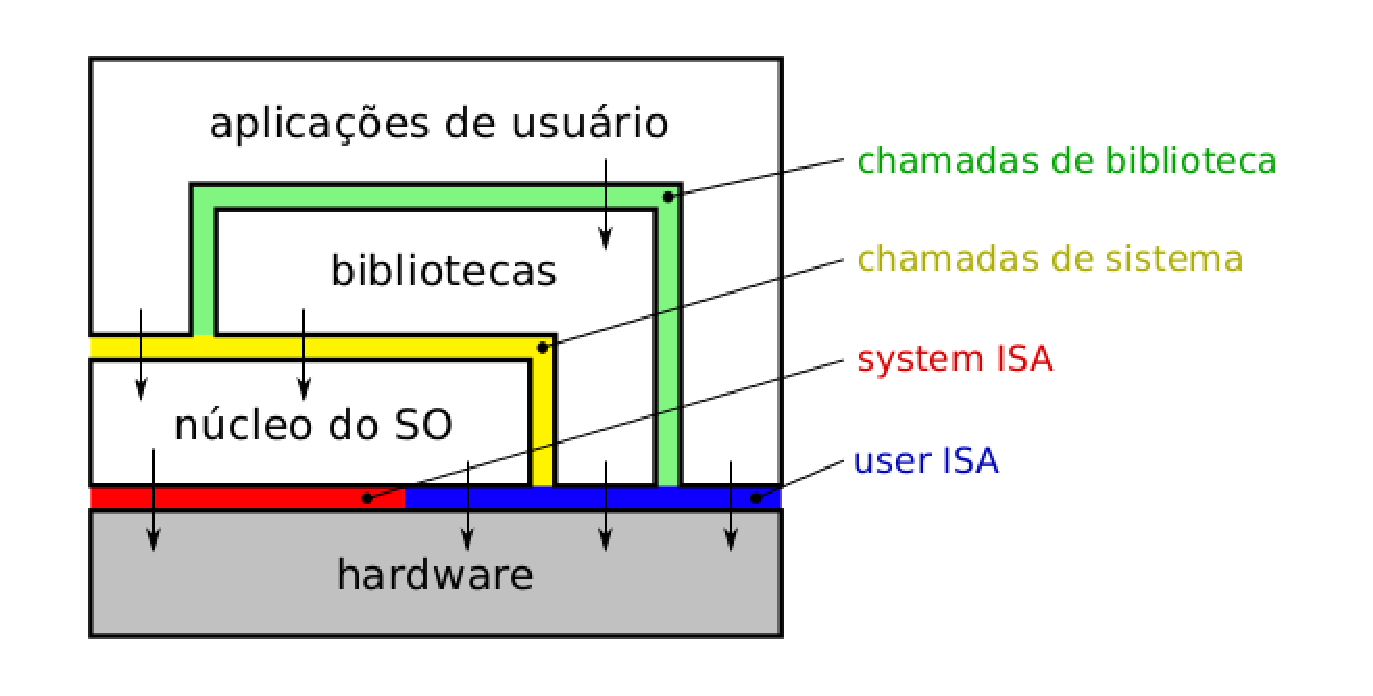
\includegraphics[width=350px]{img/interfaces_isa.eps}
 \caption{Interfaces de sistemas de computação.}
 \label{fig:interfaces_isa}
 Fonte: \citet{maziero2013}
\end{figure}

Máquinas virtuais podem ser divididas em dois grupos principais, que são: as máquinas virtuais de aplicação (Seção \ref{section:virtaplicacao}), 
e máquinas virtuais de sistema (Seção \ref{section:virtsistema}). As máquinas virtuais de aplicação fazem a virtualização de uma 
aplicação e suportam apenas um processo ou aplicação, ou seja, elas provêm um ambiente onde um sistema operacional permita a execução de
uma aplicação convidada. Um exemplo de máquina virtual de aplicação é a \ac{JVM}. Enquanto uma máquina virtual de sistema suporta um sistema
operacional convidado, com suas aplicações executando sobre ele (Figura \ref{fig:vms_tipos}). Uma máquina virtual executando sobre o 
hipervidor \ac{KVM} é um exemplo de máquina virtual de aplicação \cite{laureano2008}.

\begin{figure}[vms_tipos]
 \centering
 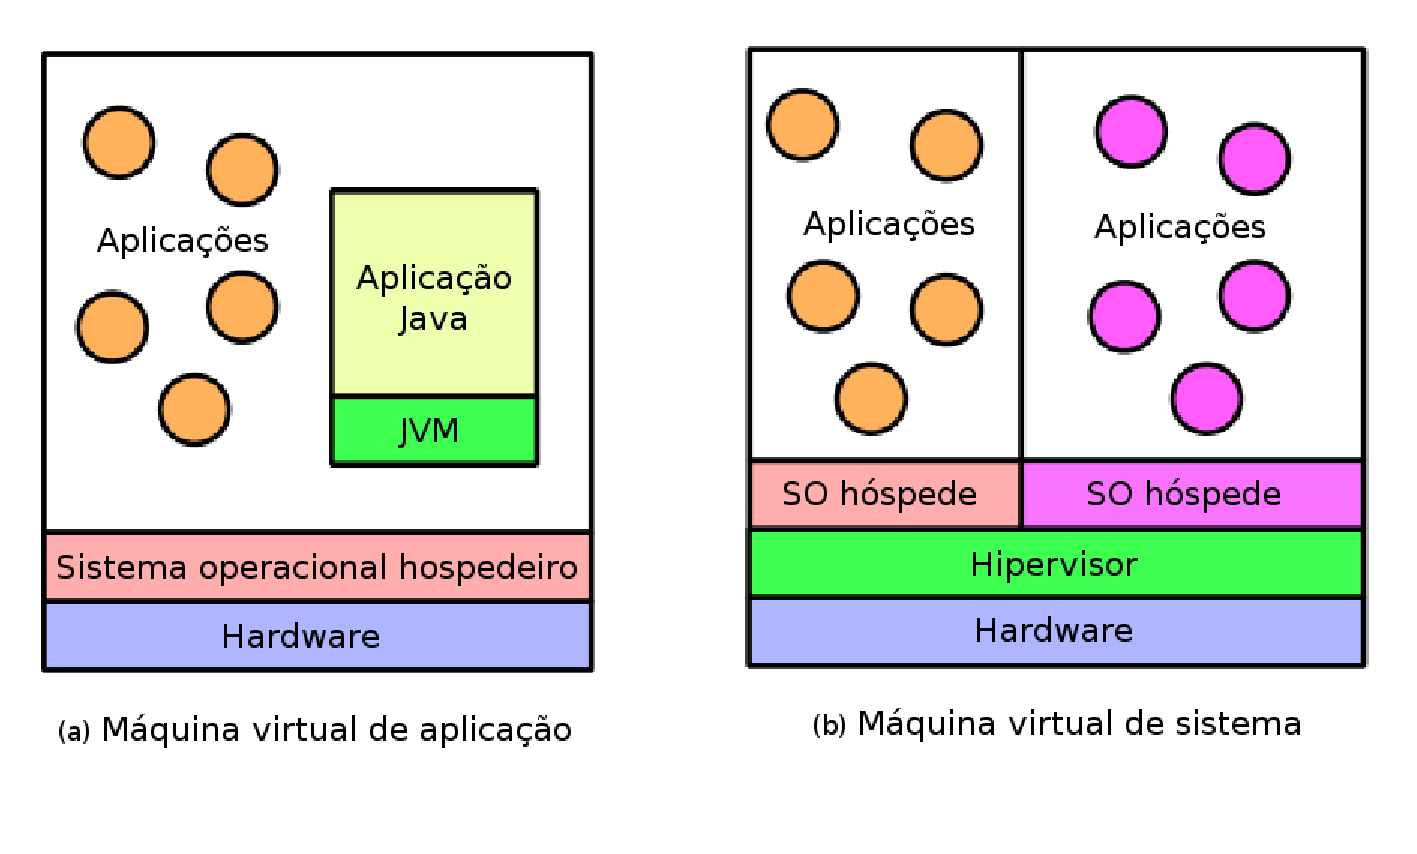
\includegraphics[width=380px]{img/vms_tipos.eps}
 \caption{Máquinas virtuais de aplicação e de sistema.}
 \label{fig:vms_tipos}
 Fonte: \citet{laureano2008}
\end{figure}

\section{Máquinas virtuais de aplicação}
\label{section:virtaplicacao}

As máquinas virtuais de aplicação, também chamadas de máquinas virtuais de processos, são responsáveis por prover um ambiente que permite 
que um sistema operacional suporte uma aplicação convidada, sendo que esta aplicação possui um conjunto de instruções, ou de chamadas
do sistema, diferentes da arquitetura do sistema hospedeiro. Neste caso, quando temos chamadas do sistema operacional ou instruções de máquina 
que são diferentes das oferecidas pela máquina real, será necessário uma tradução dessas interfaces, que será feita pela camada de 
virtualização. Os dois principais tipos de máquinas virtuais de aplicação são:

\begin{itemize}
 \item Máquinas virtuais de linguagem de alto nível: esse tipo de máquina virtual foi criado levando em consideração uma linguagem de 
 programação e o seu compilador. Neste caso, o código compilado gera um código binário que não pode ser executado em uma arquitetura real, 
 mas pode ser executado em uma máquina virtual. Sendo assim para cada arquitetura ou sistema operacional deverá existir uma máquina virtual que
 permita a execução da aplicação nesse ambiente. Como exemplo deste tipo de máquina virtual pode-se citar a máquina virtual Java (\ac{JVM})
 e a \textit{Microsoft Common Language Infrastructure}, que é a base da plataforma \textit{.NET} \cite{carissimi2008};
 \item Emulação no sistema operacional: nesse caso é feito um mapeamento entre as chamadas de sistema que são utilizadas pela aplicação 
 e as chamadas do sistema operacional real. A virtualização de aplicação pode ser encontrada em ferramentas que emulam uma aplicação 
 desenvolvida para uma plataforma em outra plataforma. Como exemplo, pode-se citar o \textit{Wine} \cite{wine}, que permite executar aplicações 
 \textit{Windows} em plataformas \textit{Linux}.
\end{itemize}

%Na virtualização de aplicação também existem máquinas virtuais que utilizam as mesmas interfaces \ac{ISA} do computador real,
%com isso uma grande parte das instruções podem ser executadas diretamente, com exceção de instruções privilegiadas, que serão devidamente
%tratadas. Alguns tipos de máquinas virtuais de aplicação que utilizam as interfaces do sistema real são:

%\begin{itemize}
% \item Sistemas operacionais multi-tarefas: sistemas operacionais que suportam simultaneamente mais de um usuário também podem ser
% vistos como máquinas virtuais. Em um sistema multi-tarefa cada processo possui um ``processador virtual'' (devido a rápida troca de 
% contextos do processador real), uma ``memória virtual'' (memória alocada para o processo) e outros recursos que podem ser acessados
% através de chamadas de sistema;
% \item Tradutores dinâmicos: esses tradutores analisam e otimizam o código de máquina para torná-lo mais eficiente. Essa otimização 
% pode ser feita durante a carga do processo na memória ou durante a execução das instruções. Pode-se citar como exemplo o \ac{JIT} 
% \textit{Bytecode compiler};
% \item Depuradores de memória: são sistemas de depuração de memória que detectam erros decorrentes do uso incorreto da memória.
% Um exemplo de depurador é o sistema \textit{Valgrind}, que utiliza uma máquina virtual para efetuar essa depuração.
%\end{itemize}

\section{Máquinas virtuais de sistema}
\label{section:virtsistema}

As máquinas virtuais de sistema, também chamadas de hipervisor ou \ac{VMM}, são uma camada de \textit{software} que possibilita
que um ou mais sistemas operacionais convidados executem independentemente sobre um mesmo computador físico. O hipervisor provê uma interface
\ac{ISA} virtual, que pode ou não ser igual a interface real, e virtualiza outros componentes de \textit{hardware}, para que cada máquina
virtual convidada possa ter seus próprios recursos.

A virtualização de sistema utiliza abstrações em sua arquitetura. Por exemplo, ela transforma um disco rígido físico em dois discos rígidos
virtuais menores, sendo que esses discos virtuais são arquivos armazenados no disco físico. Sabendo que arquivos são uma abstração
em um disco rígido físico, pode-se dizer que virtualização não é apenas uma camada de abstração do \textit{hardware}, ela faz a reprodução 
do \textit{hardware} \cite{smithenair2005}.

Nesse modelo, o ambiente de virtualização de sistema é composto basicamente por três componentes (Figura \ref{fig:virtcomponentes}):
\begin{itemize}
 \item Máquina real: também chamado de hospedeiro, que é o \textit{hardware} onde o sistema de virtualização irá executar;
 \item Camada de virtualização: é conhecida como hipervisor ou também chamada de \ac{VMM}. Essa camada tem como função criar interfaces 
 virtuais, para a comunicação da máquina virtual com a máquina real;
 \item Máquina virtual: também conhecido como sistema convidado, que executa sobre a camada de virtualização. Geralmente tem-se
 várias máquinas virtuais executando simultaneamente sobre esta camada.
\end{itemize}

\begin{figure}[virtcomponentes]
 \centering
 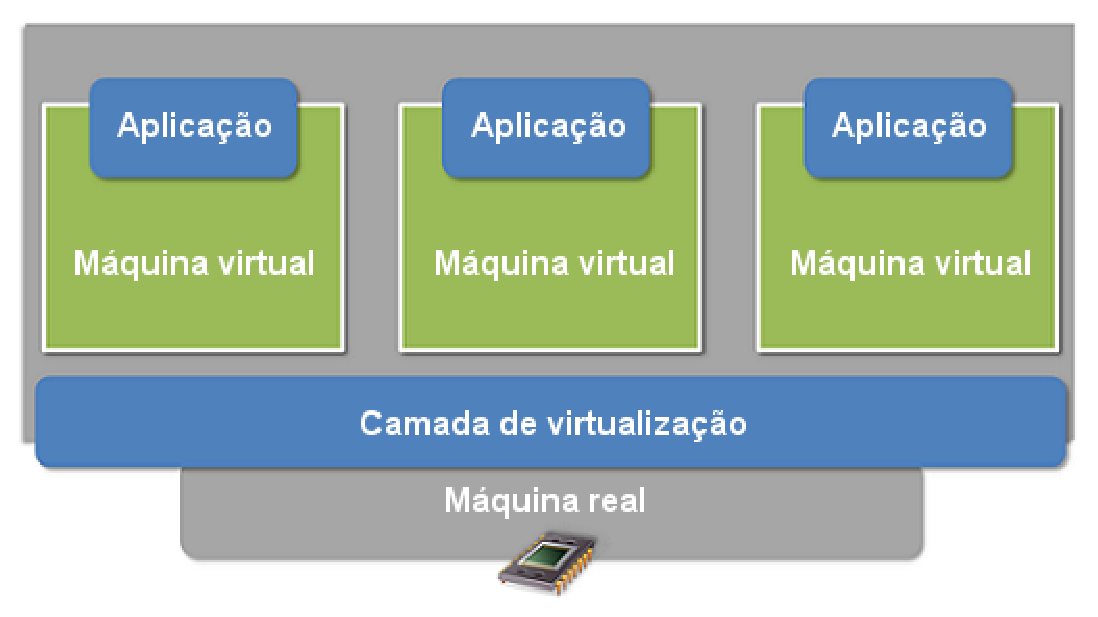
\includegraphics[width=300px]{img/virtcomponentes.eps}
 \caption{Componentes da virtualização.}
 \label{fig:virtcomponentes}
 Fonte: \citet{andrade2011}
\end{figure}

\subsection{Arquiteturas de máquinas virtuais de sistema}
\label{section:virtarquit}

Existem basicamente duas arquiteturas de hipervisor de sistema, que são apresentadas na Figura \ref{fig:vms_arquiteturas} \cite{maziero2013}:
\begin{itemize}
 \item Hipervisores nativos: esse hipervisor executa diretamente sobre o \textit{hardware}, ou seja, sem um sistema operacional
 hospedeiro. Neste caso, o hipervisor nativo faz a multiplexação dos recursos do \textit{hardware} (memória, disco rígido, interface de rede, 
 entre outros) e diponibiliza esses recursos para as máquinas virtuais. Alguns exemplos que utilizam esse hipervisor são 
 \textit{IBM 370} \cite{ibm370}, o \textit{Xen} \cite{xen} e o \textit{VMware ESXi} \cite{vmwareesxi};
 \item Hipervisores convidados: esse tipo de hipervisor executa sobre um sistema operacional hospedeiro, e utiliza os recursos 
 desse sistema para gerar recursos virtuais para as máquinas virtuais. Normalmente esse tipo suporta apenas um sistema 
 operacional convidado para cada hipervisor. Exemplos de \textit{softwares} que possuem esse tipo de arquitetura são: o 
 \textit{VirtualBox} \cite{virtualbox}, o \textit{VMware Player} \cite{vmwareplayer} e o \textit{QEmu} \cite{qemu}.
\end{itemize}

\begin{figure}[vms_arquiteturas]
 \centering
 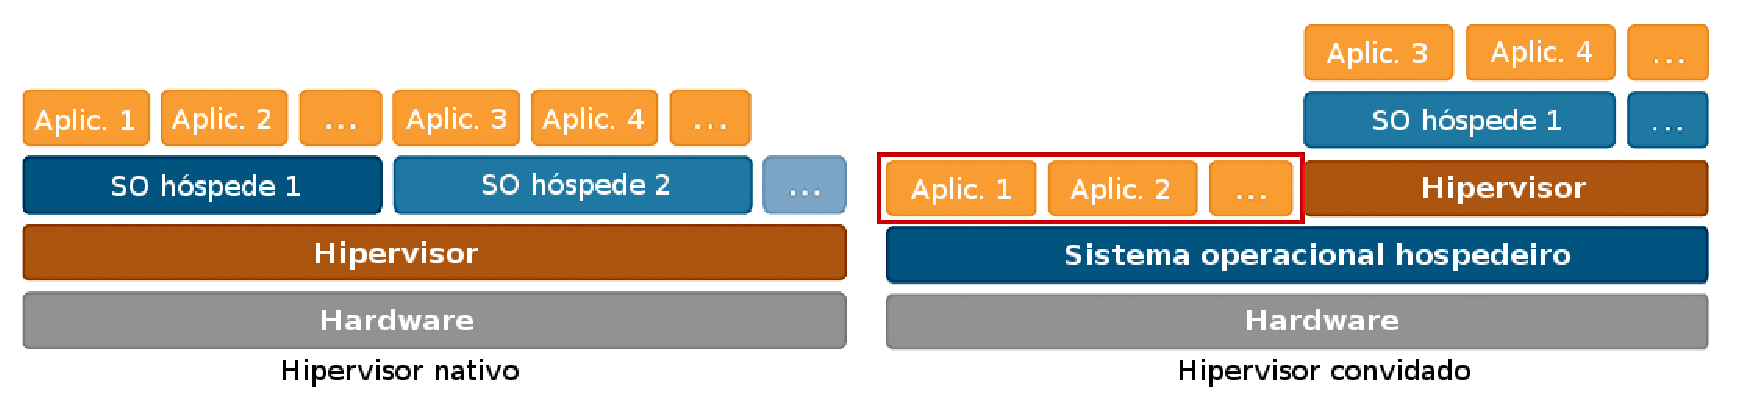
\includegraphics[width=380px]{img/vms_arquiteturas.eps}
 \caption{Arquiteturas de máquinas virtuais de sistema. COLOCAR host OS ABAIXO DO HIPERVISOR ???}
 \label{fig:vms_arquiteturas}
 Fonte: \citet{maziero2013}
\end{figure}

Destaca-se que hipervisores convidados são mais flexíveis que os nativos, pois podem ser implementados em diversos sistemas operacionais 
e \textit{hardwares}. Já os hipervisores nativos possuem melhor desempenho pois acessam o \textit{hardware} diretamente.

%\subsection{Níveis de virtualização}
%\label{section:virtniv}
%\begin{itemize}
% \item Virtualização de recursos: neste tipo de virtualização os recursos como memória e disco, além das instruções 
% privilegiadas (\textit{system \ac{ISA}}) são virtualizadas. Somente a interface \ac{ISA} de usuário é utilizada diretamente, 
% por isso o desempenho do sistema convidado é mais próximo a um sistema executando diretamente sobre um \textit{hardware}. O 
% \textit{VirtualBox} e o \textit{VirtualPC da Microsoft} são exemplos de virtualização de recursos;
% \item Virtualização completa: na virtualização completa todas interfaces são virtualizadas. Sendo assim o hipervisor fornece uma
% interface distinta ao sistema operacional convidado. Esse tipo de virtualização possui um eficiência menor, por outro lado ele
% permite executar sistemas operacionais em plataformas distintas a qual foram projetadas inicialmente. Por exemplo, o 
% \textit{MS Virtual PC for MAC}, que permite executar o sistema \textit{Windows} sobre plataforma de \textit{hardware} \textit{PowerPC}.
%\end{itemize}

%Tendo essas classificações, pode-se combiná-las para se obter quatro maneiras diferentes de implementar virtualização. Na Figura 
%\ref{fig:vms_classificacao} tem-se essas combinações com seus respectivos exemplos.

%\begin{figure}[vms_classificacao]
% \centering
% 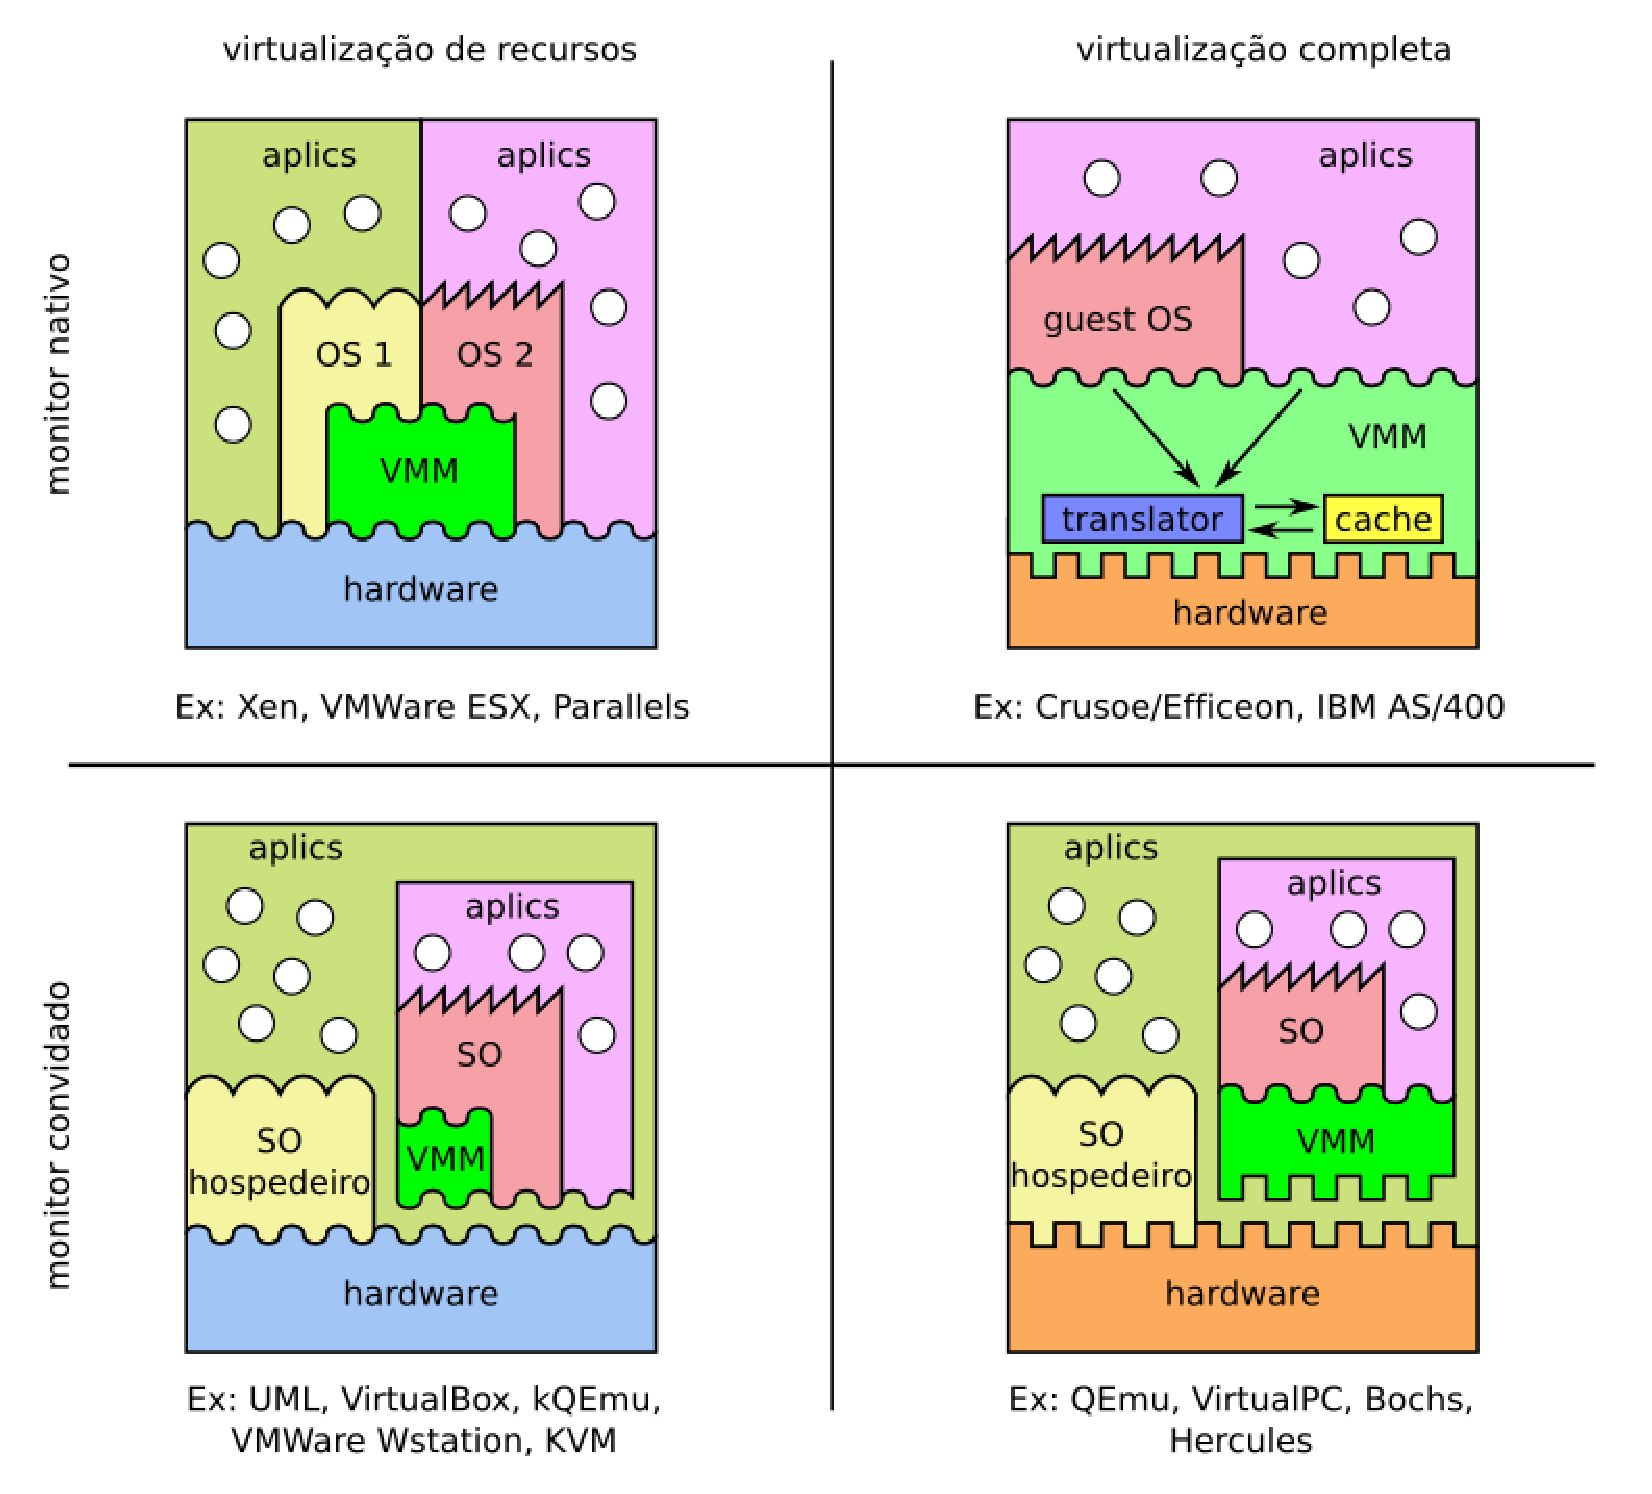
\includegraphics[width=400px]{img/vms_classificacao.eps}
% \caption{Classificação de máquinas virtuais de sistema.}
% \label{fig:vms_classificacao}
% Fonte: \citet{laureano2008}
%\end{figure}

\subsection{Implementações de máquinas virtuais de sistema}
\label{section:virtestrat}

As máquinas virtuais de sistema podem ser implementadas usando diferentes tipos de estratégias. Atualmente as estratégias mais utilizadas
são a virtualização total e a paravirtualização (Figura \ref{fig:vms_implementacao}), detalhadas a seguir:
\begin{itemize}
 \item Virtualização total: nesta estratégia todas as interfaces de acesso ao \textit{hardware} são virtualizadas. Desta forma, possibilita-se 
 que os sistemas operacionais convidados executem como se estivessem diretamente sobre o \textit{hardware}. Na virtualização total o conjunto de 
 instruções do processador é acessível somente pelo hipervisor. Sendo que essa estratégia utiliza tradução dinâmica\footnotemark[1]
 para traduzir as instruções do sistema convidado. A grande vantagem dessa estratégia é a possibilidade de um sistema convidado ser executado 
 sem a necessidade de ser modificado. Porém, essa estratégia possui um desempenho inferior devido ao fato do hipervisor intermediar todas as 
 chamadas de sistemas e operações do sistema convidado. Um exemplo ferramenta que utiliza virtualização total é o \textit{QEmu};
 \item Paravirtualização: esta utiliza arquitetura de hipervisor nativo, sendo que essa estratégia provê um melhor acoplamento entre os 
 sistemas operacionais convidados e o hipervisor. Para isso, o sistema convidado deve ser adaptado para o hipervisor no qual executará, 
 ou seja, a interface de sistema (\textit{system ISA}) será acessada diretamente pelo sistema convidado, resultando em um desempenho melhor. 
 Um exemplo de sistema que implementa a paravirtualização é o \textit{Xen}.
\end{itemize}

\begin{figure}[vms_implementacao]
 \centering
 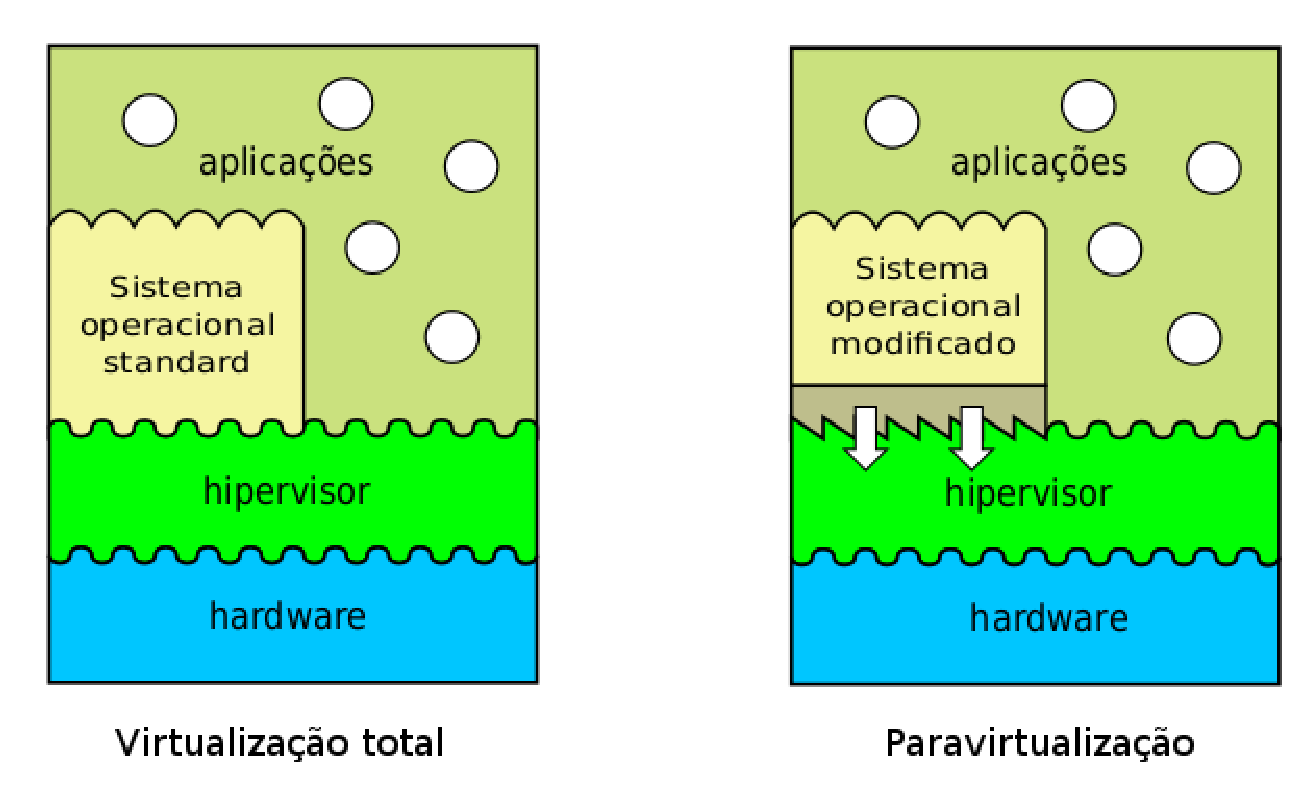
\includegraphics[width=330px]{img/vms_implementacao.eps}
 \caption{Implementações de máquinas virtuais de sistema.}
 \label{fig:vms_implementacao}
 Fonte: \citet{maziero2013}
\end{figure}

\footnotetext[1]{A tradução dinâmica analisa e reorganiza as instruções de um sistema convidado para melhorar o desempenho da execução, 
além disso a tradução dinâmica adapta as instruções do sistema convidado para o sistema real.}

A paravirtualização possui um desempenho superior se comparada a virtualização total, pois acessa alguns recursos de forma direta, sendo que 
o hipervisor é reponsável somente por impedir que o sistema convidado execute operações indevidas. Pode-se citar como exemplo o controle de
acesso à memoria feito pelo hipervisor. Na virtualização total o hipervisor reserva um espaço para cada sistema convidado, que por sua vez 
acessa a memória como se fosse uma memória física, que inicia o seu endereçamento na posição zero. Sendo assim, cada vez que o sistema convidado 
acessar a memória, o hipervisor precisará converter os endereços do sistema convidado para os endereços reais de memória. Na paravirtualização 
o hipervisor informa ao sistema convidado a área de memória que ele pode utilizar, assim não sendo necessário nenhum conversão de endereços.

Apesar de apresentar um desempenho inferior, a virtualização total possui uma maior portabilidade, ou seja, permite que sistemas operacionais 
executem como convidados, sem a necessidade de serem modificados. Pode-se, por exemplo, transferir um sistema operacional instalado diretamente 
em uma máquina física para um ambiente virtual, sem a necessidade de reinstalá-lo e reconfigurar todas as aplicações.

%A virtualização total obteve um grande ganho de performance com a incorporação da virtualização aos processadores, através das 
%tecnologias \ac{IVT} da \textit{Intel} e \ac{AMD-V} da \textit{AMD}. Elas possuem dois modos, um para execuções normais e para hipervisor, 
%e outro específico para máquinas virtuais. 

\subsection{Vantagens das máquinas virtuais de sistema}
\label{section:virtvantag}

A portabilidade é uma das grandes vantagens da virtualização, que também pode ser aplicada em \textit{desktops}. Pode-se citar como exemplo 
o desenvolvimento de \textit{software} para diversos sistemas operacionais sem a necessidade de um computador para cada sistema operacional. 
Assim, máquinas virtuais em \textit{desktops} podem ser utilizadas em ambientes de desenvolvimento, pois possibilitam a execução de múltiplas 
plataformas sem comprometer o sistema operacional original \cite{carissimi2008}. Um exemplo é o \textit{VMware Workstation}, que possibilita 
a virtualização em \ac{PC} para fins de desenvolvimento de \textit{software} \cite{vmware2016}.

Em empresas pode-se utilizar virtualização de \textit{desktops}, através da configuração de terminais remotos nos computadores e um servidor 
para centralizar as máquinas virtuais. Com isso torna-se mais simples a manutenção dos \textit{desktops} e exige um \textit{hardware} de 
menor valor, além disso essa técnica possibilita uma maior segurança dos dados. Exemplos desse tipo de virtualização são o \textit{Xen Desktop}
\cite{xendesktop} e o \textit{VMware Horizon View} \cite{vmwareview}.
%Em empresas pode-se utilizar virtualização de \textit{desktops} para reduzir a subutilização dos \textit{desktops}, que pode ser feito através da
%colaboração com projetos científicos de \textit{clusters} de computadores virtuais \cite{carissimi2008}. %exemplo seti@home

Pode-se também encontrar virtualização de \textit{desktops} em laboratórios de universidades, devido a necessidade de executar diferentes sistemas 
operacionais para determinadas disciplinas. Isso é necessário quando pretende-se configurar e executar aplicações para fim de experimentos ou
aprendizagem, com isso, essas ações não afetarão o sistema hospedeiro, pois estarão executando no sistema operacional de uma máquina virtual. 
O benefício desse tipo de cenário é a facilidade de manipulação das máquinas virtuais, pois podem ser restauradas de uma forma simples.

Em muitos casos as empresas utilizam serviços distribuídos entre diferentes servidores físicos, como, por exemplo, servidores de e-mail, 
hospedagens e banco de dados, com isso existe uma grande ociosidade de recursos. Portanto, uma das grandes vantagens da virtualização é um melhor 
aproveitamento dos recursos. De fato, alocando vários serviços em um único servidor físico tem-se um melhor aproveitamento do \textit{hardware} 
\cite{moreira2006}. Além disso, pode-se ter uma redução de custos com a administração e a manutenção dos servidores físicos. Em um ambiente 
heterogênio pode-se também utilizar virtualização, pois ela permite a instalação de diversos sistemas operacionais em um único servidor.
Esse tipo de virtualização favorece a implementação do conceito ``um servidor por serviço'', que consiste em ter um servidor para cada 
serviço. Além disso, tem-se o isolamento de serviços, ou seja, caso ocorra uma falha de segurança em um serviço, essa falha não comprometerá 
todo o sistema \cite{carissimi2008}.

Outra motivação para a utilização de virtualização consiste no custo da energia elétrica. A economia de energia pode ser obtida 
através da implantação de servidores mais robustos para substituir dezenas de servidores comuns. Outros fatores como refrigeração do ambiente e 
espaço físico utilizado também podem ser reduzidos com a implantação de virtualização de servidores, e consequentemente, reduzem os 
custos de energia.

\section{Considerações finais}

Neste Capítulo foram descritos um breve histórico e os dois principais grupos de máquinas virtuais, máquinas virtuais de aplicação e máquinas 
virtuais de sistema. Também foi apresentado as vantagens e as estratégias de implementação de máquinas virtuais de sistema. Deu-se ênfase 
para máquinas virtuais de sistema pois são o foco deste trabalho. Também pôde-se perceber que máquinas virtuais podem ser utilizadas para fazer 
redundância de \textit{software}. No próximo Capítulo será feito uma análise na empresa e a seleção dos seus serviços mais importantes para 
propor uma solução de alta diponibilidade e assim aumentar a confiabilidade dos serviços.


%\section{Emulação ????}

%Emulação é a capacidade de uma aplicação ou um dispositivo imitar um determinado conjunto de \textit{hardware}. Normalmente é
%executado como um aplicativo em um sistema operacional. A emulação é uma camada de \textit{software} que possibilita a execução
%de uma plataforma em outra plataforma distinta, com isso obtem-se a portabilidade das máquinas virtuais hospedeiras \cite{silva2009}.

%Este tipo de virtualização possui uma considerável redução de desempenho, pelo fato de toda comunicação com o \textit{hardware}
%ser intermediada pela camada de \textit{software} que faz a sua tradução. Por outro lado ela não visa desempenho, mas sim flexibilidade,
%por exemplo ela permite que desenvolvedores de \textit{firmware} e de \textit{hardware} simulem e validem aplicativos sem a presença
%do \textit{hardware} real.
